% TU Delft Beamer template
% Author: Maarten Abbink
% Delft University of Technology
% March 2014
% Version 2.0
% Based on original version 1.0 of Carl Schneider
\documentclass{beamer}
\usepackage[english]{babel}
\usepackage{calc}
\usepackage[absolute,overlay]{textpos}
\usepackage{minted}
\mode<presentation>{\usetheme{tud}}

\title[A type system for dynamic instances]{A type system for dynamic instances}
%\subtitle
\institute[TU Delft]{Delft University of Technology}
\author{Albert ten Napel}
\date{\today}

% Insert frame before each subsection (requires 2 latex runs)
\AtBeginSubsection[] {
	\begin{frame}<beamer>\frametitle{\titleSubsec}
		\tableofcontents[currentsection,currentsubsection]  % Generation of the Table of Contents
	\end{frame}
}
% Define the title of each inserted pre-subsection frame
\newcommand*\titleSubsec{Next Subsection}
% Define the title of the "Table of Contents" frame
\newcommand*\titleTOC{Outline}

\begin{document}

{
% remove the next line if you don't want a background image
\usebackgroundtemplate{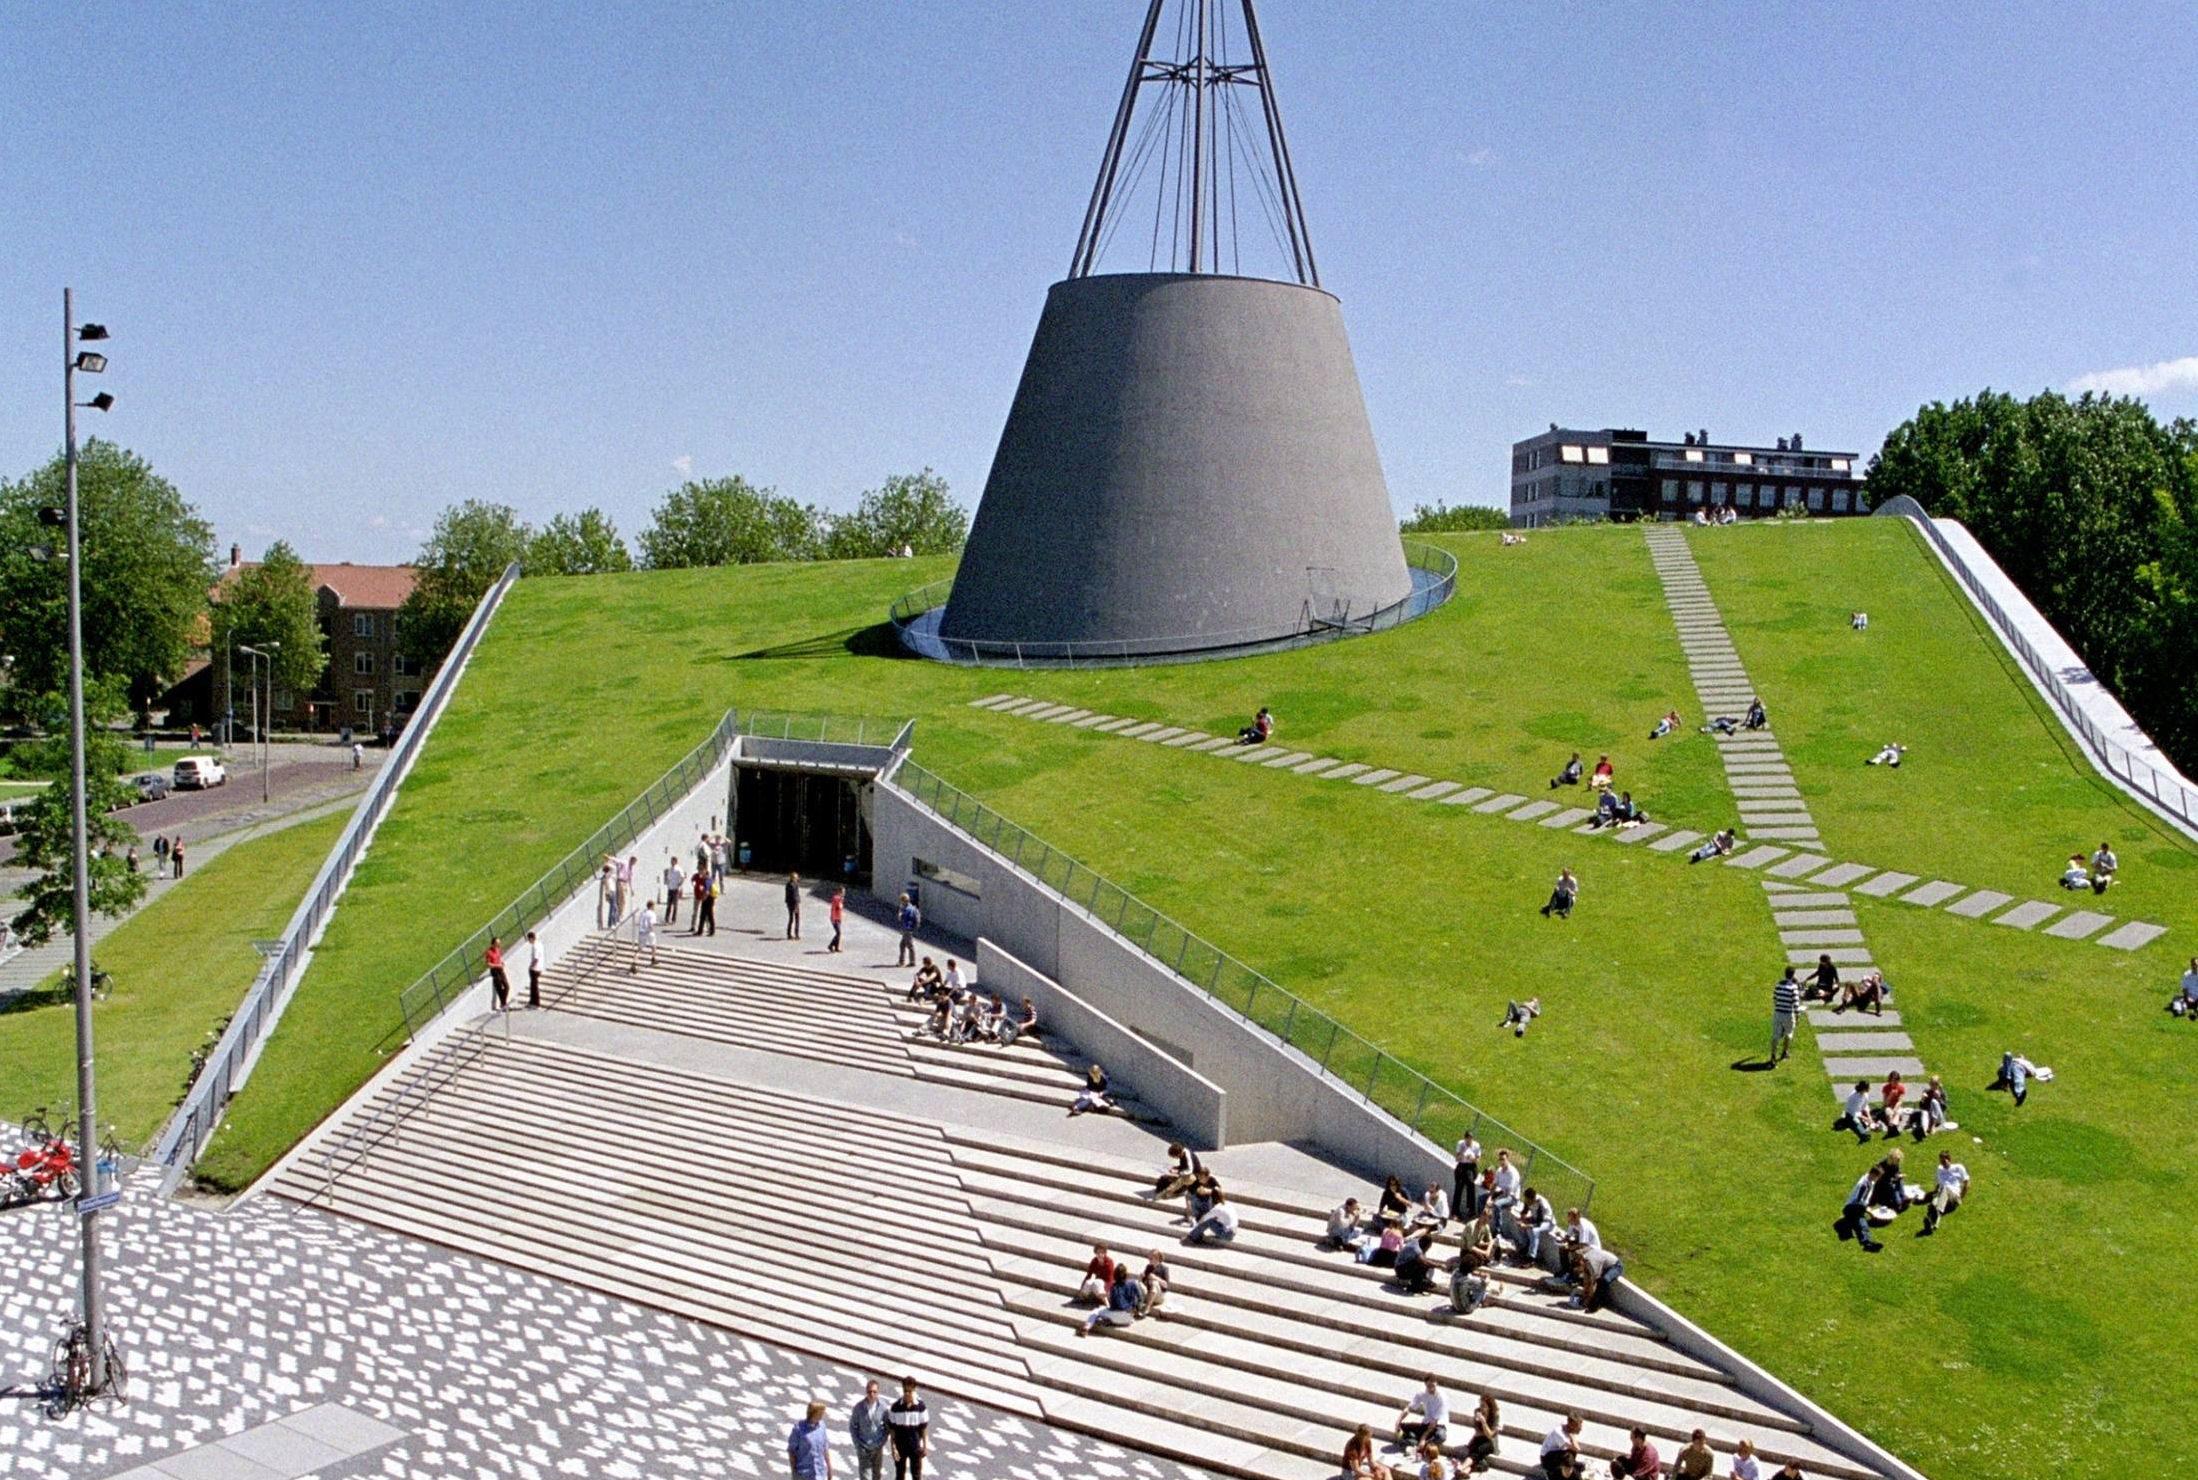
\includegraphics[width=\paperwidth,height=\paperheight]{images/background-titlepage.jpg}}%
\setbeamertemplate{footline}{\usebeamertemplate*{minimal footline}}
\frame{\titlepage}
}

{\setbeamertemplate{footline}{\usebeamertemplate*{minimal footline}}
\begin{frame}\frametitle{\titleTOC}
	\tableofcontents
\end{frame}
}

\section{Effects}

\begin{frame}[fragile]\frametitle{Effects}
	\begin{example}
		\begin{minted}{python}
guesses = 0

// guess : () -> Int
def guess():
  global guesses
  n = input("give a number: ")
  guesses += 1
  if n == "42":
    print("you guessed correctly!")
  else:
    print("wrong number")
  return guesses
		\end{minted}
	\end{example}
\end{frame}

\section{Algebraic effects and handlers}

\begin{frame}[fragile]\frametitle{Algebraic effect interfaces}
	\begin{example}
		\begin{minted}{haskell}
effect State {
  get : () -> Int
  put : Int -> ()
}

effect IO {
  input : String -> String
  print : String -> ()
}
		\end{minted}
	\end{example}
\end{frame}

\begin{frame}[fragile]\frametitle{Using algebraic effects}
	\begin{example}
		\begin{minted}{haskell}
guess : () -> Int!{State, IO}
guess () =
  n <- #input("give a number: ");
  x <- #get();
  #put(x + 1);
  if n == "42" then
    #print("you guessed correctly!")
  else:
    #print("wrong number");
  guesses <- #get();
  return guesses
		\end{minted}
	\end{example}
\end{frame}

\begin{frame}[fragile]\frametitle{Handling algebraic effects}
	\begin{example}
		\begin{minted}{haskell}
handleGuessIO : (List Int)!{State}
handleGuessIO =
  handle( guess() ) {
    input msg k -> (k "13") ++ (k "42")
    print msg k -> k ()
    return x -> return [x]
  }
		\end{minted}
	\end{example}
\end{frame}

\begin{frame}[fragile]\frametitle{Multiple state cells}
	\begin{example}
		\begin{minted}{haskell}
effect State1 {
  get1 : () -> Int
  put1 : Int -> ()
}

effect State2 {
  get2 : () -> Int
  put2 : Int -> ()
}
		\end{minted}
	\end{example}
\end{frame}

\begin{frame}[fragile]\frametitle{Dynamic effect instances}
	\begin{example}
		\begin{minted}{haskell}
r1 <- new State;
r2 <- new State;
handle#r1 (
  x <- r1#get();
  r2#put (x + 1)
) { ... }
		\end{minted}
	\end{example}
\end{frame}

\begin{frame}[fragile]\frametitle{Escaping instances}
	\begin{example}
		\begin{minted}{haskell}
escape ref =
  return \() -> ref#get ()

escaped =
  ref <- new State;
  fn <- handle#ref (escape ref) { ... };
  return fn
		\end{minted}
	\end{example}
\end{frame}

\section{Miro}

\begin{frame}[fragile]\frametitle{Miro - Creating instances}
\begin{example}
\begin{minted}[tabsize=2]{haskell}
effect Config {
  get : () -> Int
}

makeConfig : forall s. Int -> (Inst s Config)!{s}
makeConfig [s] v =
  new Config@s {
    get () k -> k v
    return x -> return x
    finally x -> x
  } as x in return x
\end{minted}
\end{example}
\end{frame}

\begin{frame}[fragile]\frametitle{Miro - Using and handling instances}
\begin{example}
\begin{minted}[tabsize=2]{haskell}
useConfig : Int
useConfig =
  runscope(myscope ->
    -- c : Inst myscope Config
    c <- makeconfig [myscope] 42;
    x <- c#get();
    return x)
\end{minted}
\end{example}
\end{frame}

\section{Syntax}

\begin{frame}[fragile]\frametitle{Miro - Syntax}
\begin{center}
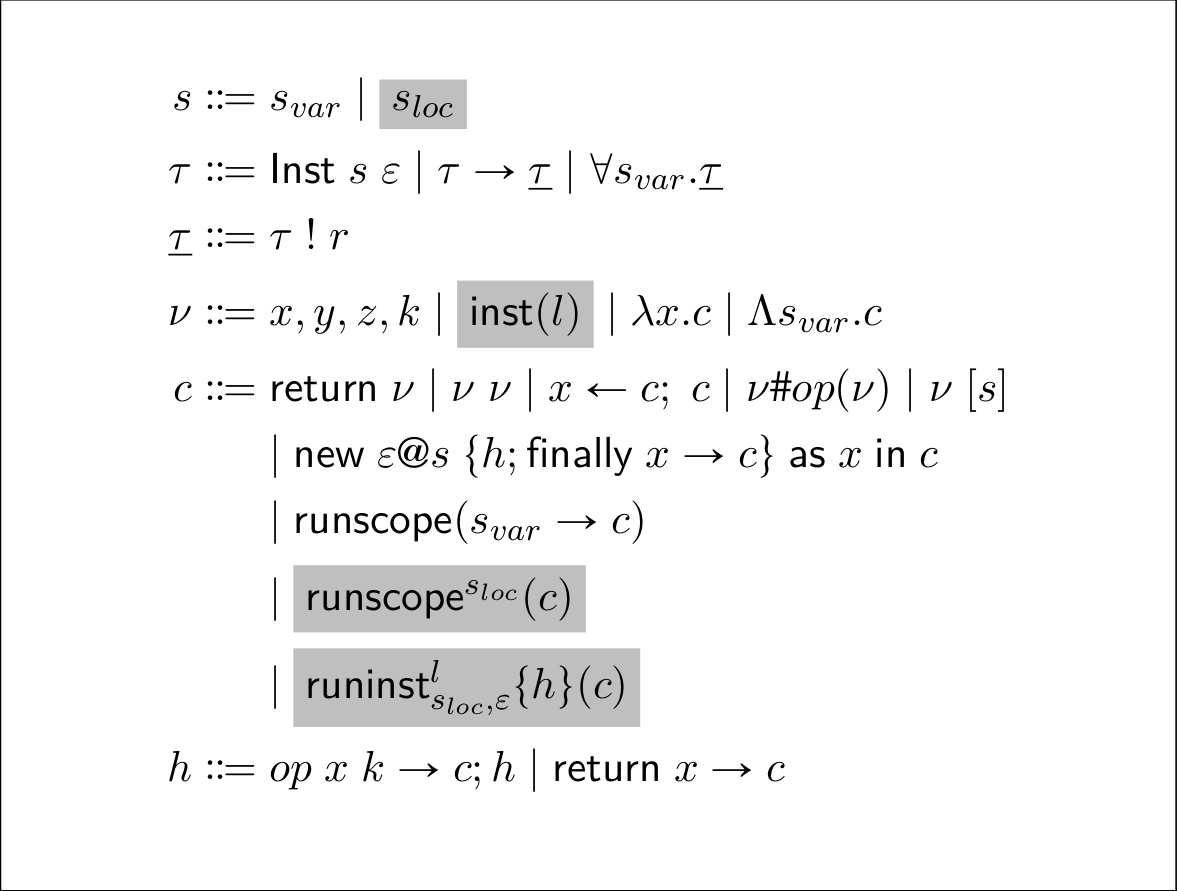
\includegraphics[width=270pt]{images/syntax.png}
\end{center}
\end{frame}

\section{Type safety}

\begin{frame}[fragile]\frametitle{Miro - Runscope typing rule}
\begin{center}
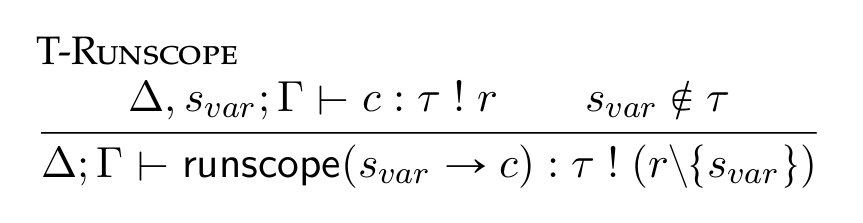
\includegraphics[width=270pt]{images/typing-rule.png}
\end{center}
\end{frame}

\begin{frame}[fragile]\frametitle{Miro - Type safety}
\begin{center}
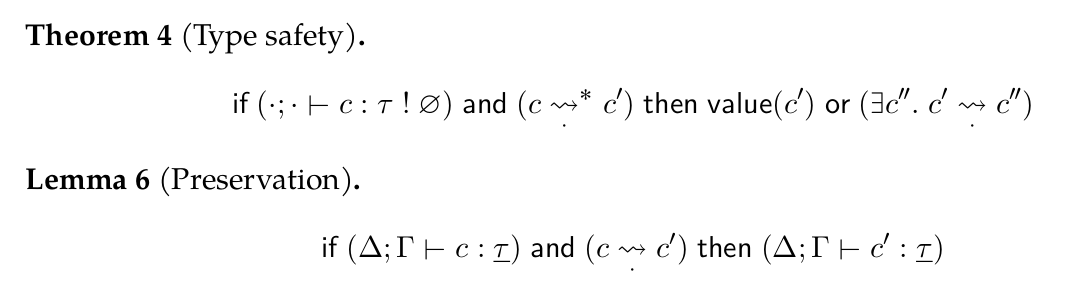
\includegraphics[width=300pt]{images/type-safety.png}
\end{center}
\end{frame}

\begin{frame}[fragile]\frametitle{Miro - Type safety issue}
\begin{center}
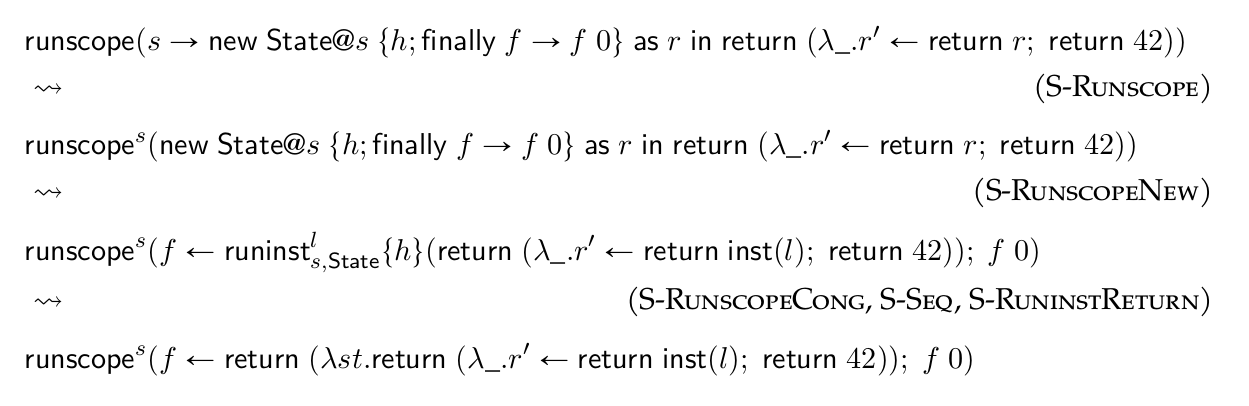
\includegraphics[width=300pt]{images/counter-example.png}
\end{center}
\end{frame}

\section{Conclusion}

\begin{frame}[fragile]\frametitle{Conclusion}
\begin{itemize}
\item A
\item B
\item C
\end{itemize}
\end{frame}

\section{Questions}

\begin{frame}[fragile]\frametitle{Questions}
Any questions?
\end{frame}

\end{document}
